\section{集合的韦恩图}

% Definition of circles
\def\firstcircle{(0,0) circle (1.5cm)}
\def\secondcircle{(0:2cm) circle (1.5cm)}

\colorlet{circle edge}{blue!50}
\colorlet{circle area}{blue!20}

\tikzset{filled/.style={fill=circle area, draw=circle edge, thick},
    outline/.style={draw=circle edge, thick}}
\begin{figure}[H]
    \centering
    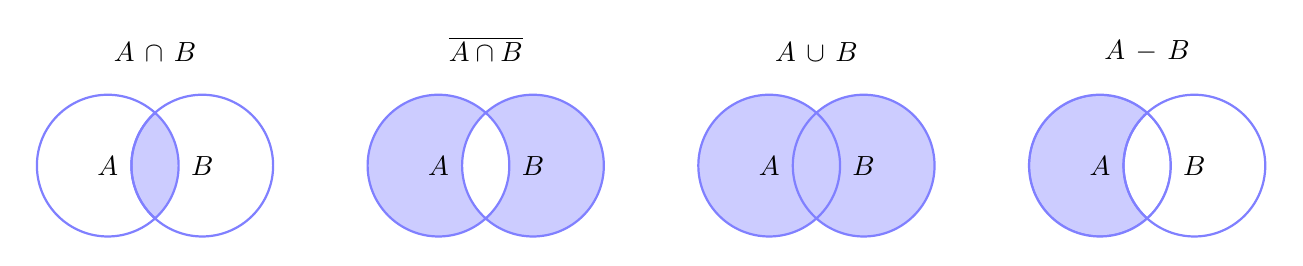
\begin{tikzpicture}[scale=0.6]
        % Set A and B
        \begin{scope}[xshift=0cm]
            \begin{scope}
                \clip \firstcircle;
                \fill[filled] \secondcircle;
            \end{scope}
            \draw[outline] \firstcircle node {$A$};
            \draw[outline] \secondcircle node {$B$};
            \node[anchor=south, text width=3cm, align=center] at (1,2) {$A \cap B$};
        \end{scope}

        % Set not(A and B)
        \begin{scope}[xshift=7cm]
            \draw[filled, even odd rule] \firstcircle node {$A$}
            \secondcircle node{$B$};
            \node[anchor=south, text width=3cm, align=center] at (1,2) {$\overline{A \cap B}$};
        \end{scope}

        % Set A or B
        \begin{scope}[xshift=14cm]
            \draw[filled] \firstcircle node {$A$}
            \secondcircle node {$B$};
            \node[anchor=south, text width=3cm, align=center] at (1,2) {$A \cup B$};
        \end{scope}

        % Set A but not B
        \begin{scope}[xshift=21cm]
            \begin{scope}
                \clip \firstcircle;
                \draw[filled, even odd rule] \firstcircle node {$A$}
                \secondcircle;
            \end{scope}
            \draw[outline] \firstcircle
            \secondcircle node {$B$};
            \node[anchor=south, text width=3cm, align=center] at (1,2) {$A - B$};
        \end{scope}
    \end{tikzpicture}
\end{figure}

\begin{example}
    设全集 $U=\left\{x \mid x<10, x \in \mathbf{N}^*\right\}$ ，集合 $A, B \subseteq U$ ，若 $A \cap B=\{3\}, A \cap\left(\mathrm{C}_U B\right)=\{1,5,7\},\left(\mathrm{C}_U A\right) \cap\left(\mathrm{C}_U B\right)=\{9\}$ ，则 （\qquad）
    \begin{tasks}(3)
        \task $A=\{1,3,5,7\}$
        \task $B=\{2,4,6,8\}$
        \task $9 \notin(A \cup B)$
    \end{tasks}
\end{example}

\begin{solution}
    \begin{figure} [H]
        \centering
        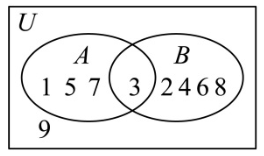
\includegraphics[width=0.2\textwidth]{chapters/集合/images/韦恩图/img-20250803195554.png}
    \end{figure}
\end{solution}


\begin{tips}
    上述容斥原理问题使用韦恩图解决最快。
\end{tips}

\begin{center}
    \begin{tikzpicture}[scale=0.7]
        \definecolor{myred}{RGB}{255,150,150}
        \definecolor{mygreen}{RGB}{150,255,150}
        \definecolor{myblue}{RGB}{150,150,255}
        \draw[fill=myred, opacity=0.6] (0, 0) circle (2.5cm);
        \draw[fill=mygreen, opacity=0.6] (-2.1, -3) circle (2.5cm);
        \draw[fill=myblue, opacity=0.6] (2.1, -3) circle (2.5cm);
        \node at (0, 1) {只A};
        \node at (-2.1, -3) {只B};
        \node at (2.1, -3) {只C};
        \node at (-1.2, -1.5) {只AB};
        \node at (1.2, -1.5) {只AC};
        \node at (0, -3.5) {只BC};
        \node at (0, -2) {ABC};
    \end{tikzpicture}
\end{center}